\subsection{Problem}
\label{subsec:problem}

% - More general about architectural patterns in the presentation layer
%    - why?
%    - what exists?
%    - state managment in general?
%    - then mvi 
%        - short explanation
%        - relatively new
%        - existing solutions
%            - do they have problems?
%    - there is no standaized way to do it
%    - android specific problems?

Applications today have increased in complexity compared to its counterpart just a few years ago. Especially in the field of frontend development the amount of 
functions has increased
\cite{increasingNatureOfFrontendKevinBall2018}. 
The web development has transitioned from server rendered, 
page-reloading websites, to modern so called single page applications or SPA's.
The same applies to the mobile world: social networks, navigation, sharing and editing files together is a common want by the user.
A large part of applications are thus interacting with APIs, accessing local or external databases
and communicating with the underlying operating system itself (eg the periodic recording of the location via GPS or Wi-Fi).
\\
\\
The challenge a developer faces is to come up with a general approach that bridges the gap between what the users sees and the source code of 
the application - mainly: How to structure the user facing parts of the codebase also known as the presentation layer
\cite{patternsOfEnterpriseApplicationArchitectureMartinFowlerPresentationLayer,softwareArchitecturePatternMarkRichards2015PresentationLayer} 
in a layered architecture.
\cite{threeTierArchitectureDonaldWolfe2013}.
\\
\\
Like many other problems in software development, this one is a problem that has existed for quite some time and concerns a large part of the developers.
It is therefore a common problem. This often results in the endeavour to develop a universally valid concept that counteracts these problems and points out 
possible solutions. The sought out concept here is defined as an "architectural" pattern.
\cite{softwareArchitecturePatternMarkRichards2015, patternOrientedSoftwareArchitectureFrankBuschmann2007, designPatternElementsOfErichGamma2000}
Its goal is to lay out a structure and architecture of source code in such a way that it is modular, flexible and
reusable. At the same time, the developer is invited to follow a pattern and produce consistent and readable code. This promotes quality and
maintainability of the application. Over time, many "architectural" patterns have evolved for structuring code within the presentation layer. 
These include, among others, the following, sorted in ascending order by year of publication: Model-View-Controller (MVC - 1979) 
\cite{theModelViewEditorTrygveReenskaug1979,modelsViewsControllersTrygveReenskaug1979,aDescriptionOfTheModelViewControllerGlennE1988,professionalASPNETMVC52014}, 
Model-View-Presenter (MVP - 1996) 
\cite{mVPModelViewPresenterTheTaligentMikePotel1996,modelViewPresenterMartinFowler2006,proAspNetMVC3FrameworkModelViewPresenter2011},
Model-View-ViewModel (MVVM) 
\cite{introductionToModelViewModelPatternJohnGossman2005, modelViewViewModelDesignPatternUsingWindowsErikSorenson2010,proAspNetMVC3FrameworkModelViewPresenter2011}
und - relatively new to the group - Model-View-Intent (MVI - 2015) 
\cite{whatIfTheUserWasAFunctionYoutubeAndreStaltzUserFunction2015,reactiveProgrammingWithRxJSMVISergiMansilla,modelViewIntentOnAndroidHannesDorfmann2016}. 
Each of the patterns listed here serves the same purpose: the strict separation of the user interface from the underlying (business) logic.
\\
\\




























MVI also makes use of this idea. Brought to life by André (Medeiros) Staltz, MVI encapsulates the interaction between the user and the application as a cycle 
(as shown in figure 
\ref{fig:userComputerInputOutput}), 
where the data flows unidirectionally 
\cite{unidirectionalDataFlowFluxArchitectureIlyGelman2017,unidirectionalDataFlowTamingTheStateinReactRobinWieruch2018,unidirectionalDataFlowTheCompleteReduxBookIlyGelman2017}.
It takes its inspiration from three concepts: The original MVC as introduced by Trygve Reenskaug in 1979, the JavaScript framework Redux 
\cite{reduxReduxQuickStartGuidJamesLee2019} 
and the JavaScript library React 
\cite{reactJSReactJsAnOpenSourceNaimulIslamNaim2017}. 
The idea of a cycle is based on the assumption that the output (e.g. a click) from a user resembles the input for the program. The program in turn produces an output 
which becomes the input for the user.
\begin{figure}[ht]
    \centering
    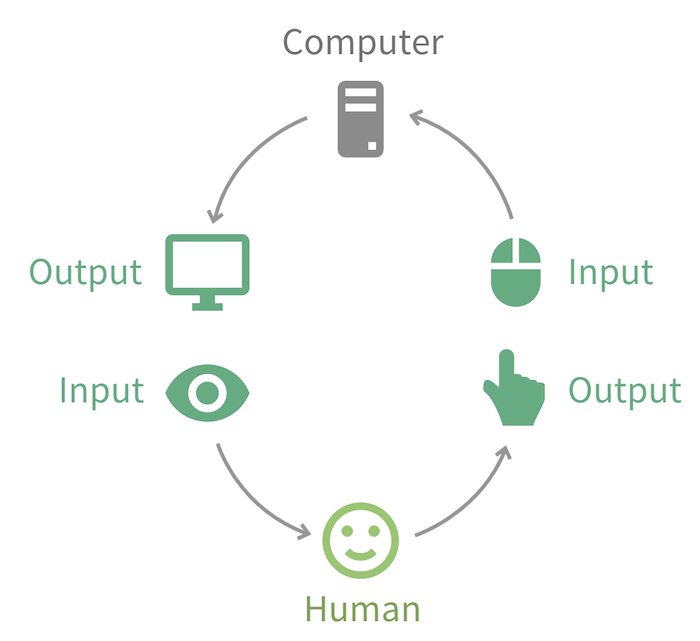
\includegraphics[height=0.5\textwidth]{./images/mvi-cycle}
    \caption{User and Computer as Input and Output}
    \caption*{Source: https://cycle.js.org/dialogue.html}
    \label{fig:userComputerInputOutput}
\end{figure}
This concept can be embodied as a chain of mathematical functions: f(g(a())) or view(model(intent(event))).
When the user interface registers an event (e.g. a click) it will be passed to the intent functions as a parameter. 
The purpose of the intent-function is to translate the user generated event into something the application can understand and work with.
In addition, the event contains data that is necessary for further processing. This requires the event to be accurately described, unique and expressive.
The model function then consumes the output (intent function) as its input. Its job is it to create a new model without changing the last one. 
That's what is referred to as immutability. 
\cite{immutabilityEffectiveJavaJoshuaBloch2017,immutabilityImmutableObjectsInJavaChristianHaack2006}
It's a concept that belongs (but is not exclusive) to a programming paradigm called functional programming
\cite{functionalProgrammingFunctionalProgrammingInJavaPierreYves2017},
where MVI adopts some of its ideas from.
\\
Finally the view function receives the model as its input and takes care of rendering it (a visual representation of the model for the user). 
In order to achieve the cycle effect and the unidirectional data flow, MVI makes use of reactive programming 
\cite{reactiveProgrammingReactiveProgrammingWithJavaBenChristensen,reactiveProgrammingTheIntroductionToReactiveAndreStaltz} 
and the underlying "Observer" pattern 
\cite{}.
To quote Andre Staltz:
\begin{pquotation}{\cite{citationMVIAndreStaltz}, Andre Staltz}
    Model-View-Intent (MVI) is reactive, functional, and follows the core idea in MVC. It is reactive because Intent observes the User, Model observes the Intent, 
    View observes the Model, and the User observes the View. It is functional because each of these components is expressed as a referentially transparent function 
    over streams. It follows the original MVC purpose because View and Intent bridge the gap between the user and the digital model, each in one direction.
\end{pquotation}
Due to MVI being based on functional paradigms and hence using pure functions, it has to fight a common problem in applications called "side effects".
As mentioned above, it is ofen a requirement to access APIs or a local database, but calling them inside of a pure function is technically not allowed.
\todo{why reactive, what does reactive solve for MVI? Streams? state?}
\\
Given this description of MVI and the mentioned problems, the questions that arise are: What does an event look like? How is immutability achieved?
Since MVI does not have a "Controller", "Presenter" or a "ViewModel": Where does the user user-interface logic belong? And how is separation of concerns possible?
To summarize, it becomes a question of implementation and design. What does a developer have to do in order to implement or reap the benefits from this concept of MVI?




